\section{Resoconto attività di verifica}
In questa sezione sono descritte le attività di verifica svolte sui documenti che vengono presentati alle revisioni di avanzamento. Qualora una verifica riscontrasse un problema su un documento, nella sezione \S C si discuterà di quali siano i possibili miglioramenti.
Inoltre verranno utlizzate delle sigle per fare riferimento al periodo in cui sono stati rilevati i risultati delle verifiche. Le sigle sono le seguenti:
\begin{itemize}
\item \textbf{An}: Analisi;
\item \textbf{TB}: Technology Baseline;
\item \textbf{PB}: Product Baseline;
\item \textbf{VC}: Validazione e Collaudo. 
\end{itemize}

\subsection{Analisi dei documenti}
\subsubsection{Analisi statica}
L'analisi dei documenti mediante Walkthrough (vedi \textit{Norme di Progetto}) ha portato all'individuazione di alcuni errori frequenti a partire dai quali è stata stilata una check list. In questo modo sarà possibile applicare l’Inspection (vedi \textit{Norme di Progetto}) per le future attività di verifica.


\paragraph{Esiti Indice di Gulpease} \mbox{} \\
\begin{longtable}{c c c c c c}
\rowcolor{white}\caption{Esiti verifica documenti con Indice di Gulpease} \\
		\rowcolor{redafk}
\textcolor{white}{\textbf{Documento}} &
\textcolor{white}{\textbf{An}} &
\textcolor{white}{\textbf{TB}} &
\textcolor{white}{\textbf{PB}} &
\textcolor{white}{\textbf{VC}} &
\textcolor{white}{\textbf{Esito}} \\
		\endfirsthead
		\rowcolor{white}\caption[]{(continua)} \\
		\rowcolor{redafk}
\textcolor{white}{\textbf{Documento}} &
\textcolor{white}{\textbf{An}} &
\textcolor{white}{\textbf{TB}} &
\textcolor{white}{\textbf{PB}} &
\textcolor{white}{\textbf{VC}} &
\textcolor{white}{\textbf{Esito}} \\
		\endhead
		\textit{Analisi dei Requisiti} & 70 & 73 & - & - & Superato \\
		\textit{Glossario} & 74 & 74 & - & - & Superato \\
		\textit{Norme di Progetto} & 67 & 69 & - & - & Superato \\
		\textit{Piano di Progetto} & 69 & 71 & - & - & Superato \\
		\textit{Piano di Qualifica} & 72 & 71 & - & - & Superato \\
		\textit{Studio di Fattibilità} & 70 & - & - & - & Superato \\
		\textit{Media Verbali} & 71 & 74 & - & - & Superato\\
\end{longtable}

\begin{figure}[H]
\centering
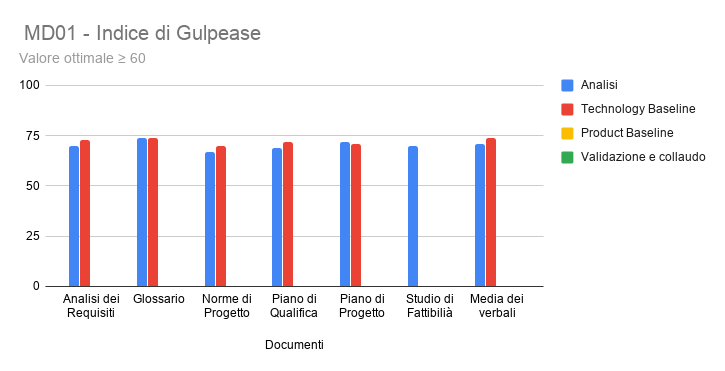
\includegraphics[scale=0.5]{./img/MD01_gulpease.png}
\caption{Grafico relativo ai dati di MD01 - Indice di Gulpease}
\end{figure}

\paragraph{Esiti Indice Fog} \mbox{} \\
\begin{longtable}{c c c c c c}
\rowcolor{white}\caption{Tabella Indice Fog} \\
		\rowcolor{redafk}
\textcolor{white}{\textbf{Attività}} &
\textcolor{white}{\textbf{An}} &
\textcolor{white}{\textbf{TB}} &
\textcolor{white}{\textbf{PB}} &
\textcolor{white}{\textbf{VC}} &
\textcolor{white}{\textbf{Riscontro}}  \\
		\endfirsthead
		\rowcolor{white}\caption[]{(continua)} \\
		\rowcolor{redafk}
\textcolor{white}{\textbf{Attività}} &
\textcolor{white}{\textbf{An}} &
\textcolor{white}{\textbf{TB}} &
\textcolor{white}{\textbf{PB}} &
\textcolor{white}{\textbf{VC}} &
\textcolor{white}{\textbf{Riscontro}}  \\
		\endhead
\textit{Analisi dei Requisiti} & 18 & 17 & - & - & Accettabile\\
\textit{Glossario} & 15 & 15 & - & - & Accettabile \\
\textit{Norme di Progetto} & 20 & 18 & - & - & Accettabile\\
\textit{Piano di Progetto} & 18 & 20 & - & - & Accettabile\\
\textit{Piano di Qualifica} & 20 & 20 & - & - & Accettabile\\
\textit{Studio di Fattibilità} & 14 & - & & & Accettabile\\
\textit{Media Verbali} & 8 & 6 & - & - & Ottimale\\
\end{longtable}

\begin{figure}[H]
\centering
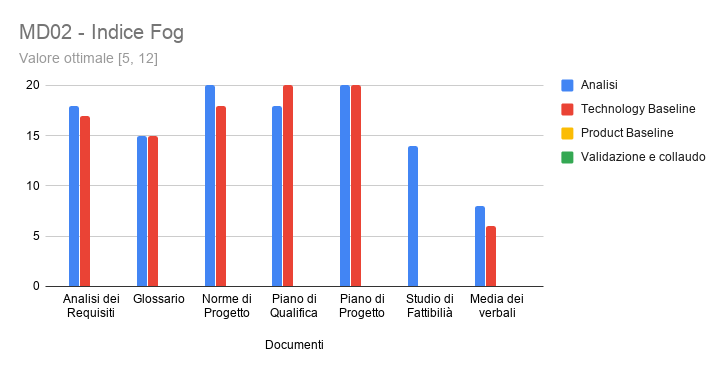
\includegraphics[scale=0.5]{./img/MD02_fog.png}
\caption{Grafico relativo ai dati di MD02 - Indice Fog}
\end{figure}

\subsection{Analisi dei processi}
\subsubsection{Esiti MP01 - Schedule Variance} 
\begin{longtable}{c c c c c c}
\rowcolor{white}\caption{Esiti verifica Schedule Variance} \\
		\rowcolor{redafk}
\textcolor{white}{\textbf{Attività}} &
\textcolor{white}{\textbf{An}} &
\textcolor{white}{\textbf{TB}} &
\textcolor{white}{\textbf{PB}} &
\textcolor{white}{\textbf{VC}} &
\textcolor{white}{\textbf{Riscontro}} \\
		\endfirsthead
		\rowcolor{white}\caption[]{(continua)} \\
		\rowcolor{redafk}
\textcolor{white}{\textbf{Attività}} &
\textcolor{white}{\textbf{An}} &
\textcolor{white}{\textbf{TB}} &
\textcolor{white}{\textbf{PB}} &
\textcolor{white}{\textbf{VC}} &
\textcolor{white}{\textbf{Riscontro}} \\
		\endhead
\textit{Analisi dei Requisiti} & 
1 &
1 &
- &
- &
Accettabile \\
\textit{Glossario} & 
0 &
0 &
- &
- &
Ottimale \\
\textit{Norme di Progetto} & 
0 &
1 &
- &
- &
Accettabile \\
\textit{Piano di Qualifica} & 
1 &
-2 &
- &
- &
Ottimale \\
\textit{Piano di Progetto} & 
1 &
0 &
- &
- &
Ottimale \\
\textit{Studio di Fattibilià} & 
0 &
- &
- &
- &
Ottimale \\
\end{longtable}

\begin{figure}[H]
\centering
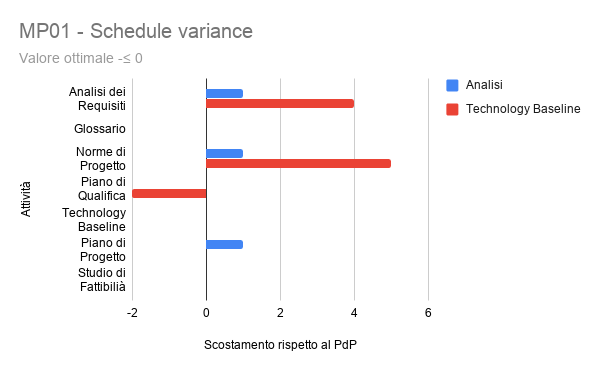
\includegraphics[scale=0.6]{./img/MP01_schedule_variance.png}
\caption{Grafico relativo ai dati di MP01 - Schedule Variance}
\end{figure}

\subsubsection{Esiti MP02 - Budget Variance}
\begin{longtable}{c c c c c}
\rowcolor{white}\caption{Esiti Budget Variance} \\
		\rowcolor{redafk}
\textcolor{white}{\textbf{An}} &
\textcolor{white}{\textbf{TB}} &
\textcolor{white}{\textbf{PB}} &
\textcolor{white}{\textbf{VC}} &
\textcolor{white}{\textbf{Riscontro}} \\
-8,66$\%$ &
-1,19$\%$ &
- &
- &
Accettabile \\
\end{longtable}

\begin{figure}[H]
\centering
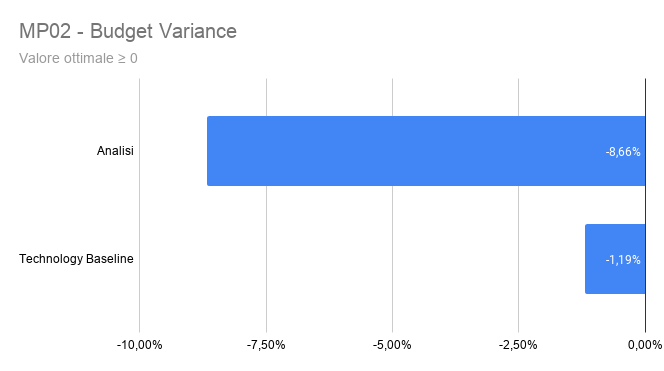
\includegraphics[scale=0.5]{./img/MP02_budget_variance.png}
\caption{Grafico relativo ai dati di MP02 - Budget Variance}
\end{figure}

\subsubsection{Esiti MP03 - Produttività} 
\begin{longtable}{c c c c c c}
\rowcolor{white}\caption{Esiti della Produttività} \\
		\rowcolor{redafk}
\textcolor{white}{\textbf{Membro}} &
\textcolor{white}{\textbf{An}} &
\textcolor{white}{\textbf{TB}} &
\textcolor{white}{\textbf{PB}} &
\textcolor{white}{\textbf{VC}} &
\textcolor{white}{\textbf{Riscontro}} \\
		\endfirsthead
		\rowcolor{white}\caption[]{(continua)} \\
		\rowcolor{redafk}
		\textcolor{white}{\textbf{Membro}} &
\textcolor{white}{\textbf{An}} &
\textcolor{white}{\textbf{TB}} &
\textcolor{white}{\textbf{PB}} &
\textcolor{white}{\textbf{VC}} &
\textcolor{white}{\textbf{Riscontro}} \\
		\endhead
Simone Federico Bergamin & 0 & 78 & - & - & Accettabile\\
Alessandro Canesso & 0 & 139 & - & - & Ottimale \\
Victor Dutca & 0 & 108 & - & - & Ottimale \\
Fouad Farid & 0 & 109 & - & - & Ottimale \\
Simone Meneghin & 0 & 93 & - & - & Accettabile\\
Olivier Utshudi & 0 & 93 & - & - & Accettabile\\
Davide Zillio & 0 & 93 & - & - & Accettabile

\begin{comment}
Metterei una nota a pié di pagina per spiegare che i valori sono a consuntivo e per questo, non sono alcuni componenti hanno scritto codice che in realtà non dovevano
\end{comment}
\end{longtable}


\begin{figure}[H]
\centering
\includegraphics[scale=0.5]{./img/MP03_produttività.png}
\caption{Grafico relativo ai dati di MP03 - Produttività}
\end{figure}